RF, LUCCK, and SVM were trained on tensor-reduced ECG features, presented in Table \ref{fig:ecgonly}. We compare these models to those trained on tensor-reduced ECG features and arterial line features, presented in Table \ref{fig:sigonly}. These figures display the mean F1 Score and AUROC over 100 iterations, with error bars indicating one SD. The $x$-axis indicates the rank selected for CP-ALS, with the rightmost columns, separated with a dashed line, representing the case where no tensor decomposition was applied.

Figure \ref{fig:sigEHR} shows the results of models trained on both the tensor-reduced signal features and EHR data.

\begin{figure}[htb]
    \centering
    \begin{subfigure}[htb]{\textwidth}
        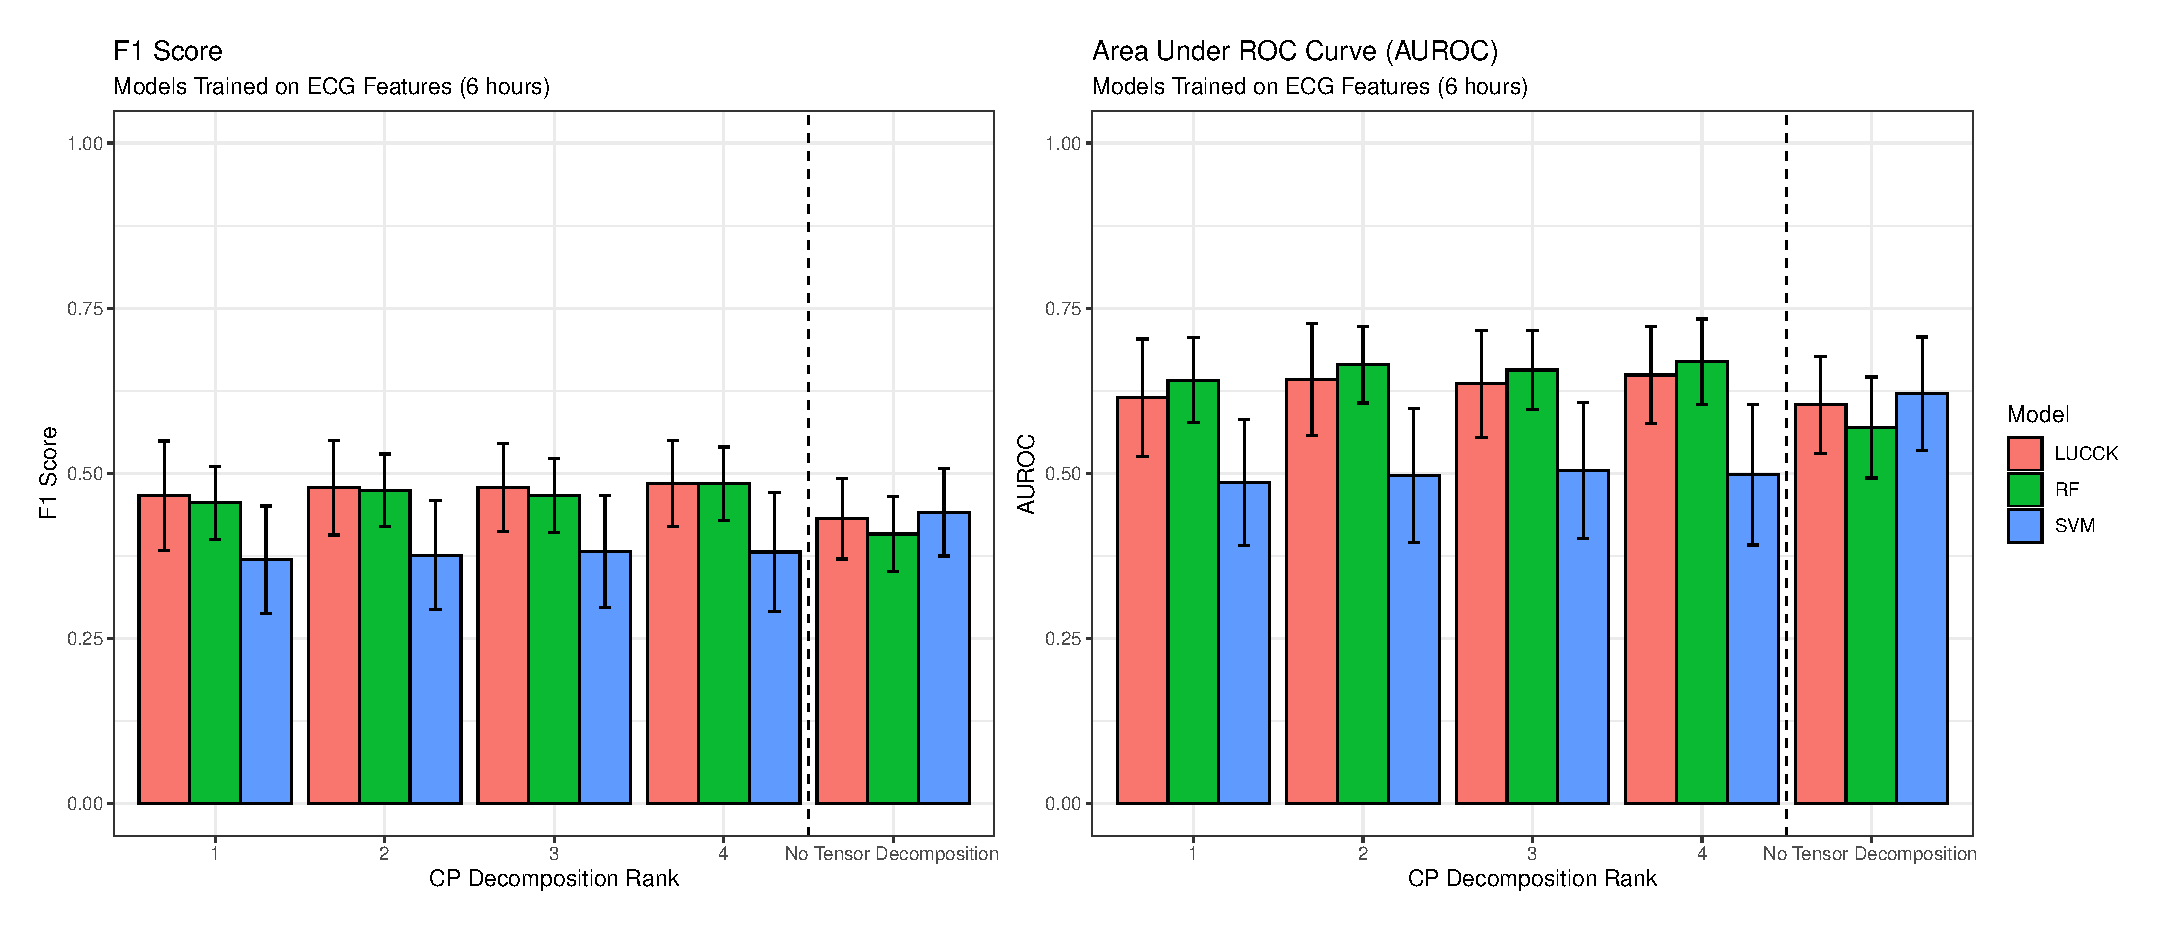
\includegraphics[width=\textwidth]{body/figures/ecg_6.eps}
        \caption{6-hour data}
    \end{subfigure}
    \hfill
    \begin{subfigure}[htb]{\textwidth}
        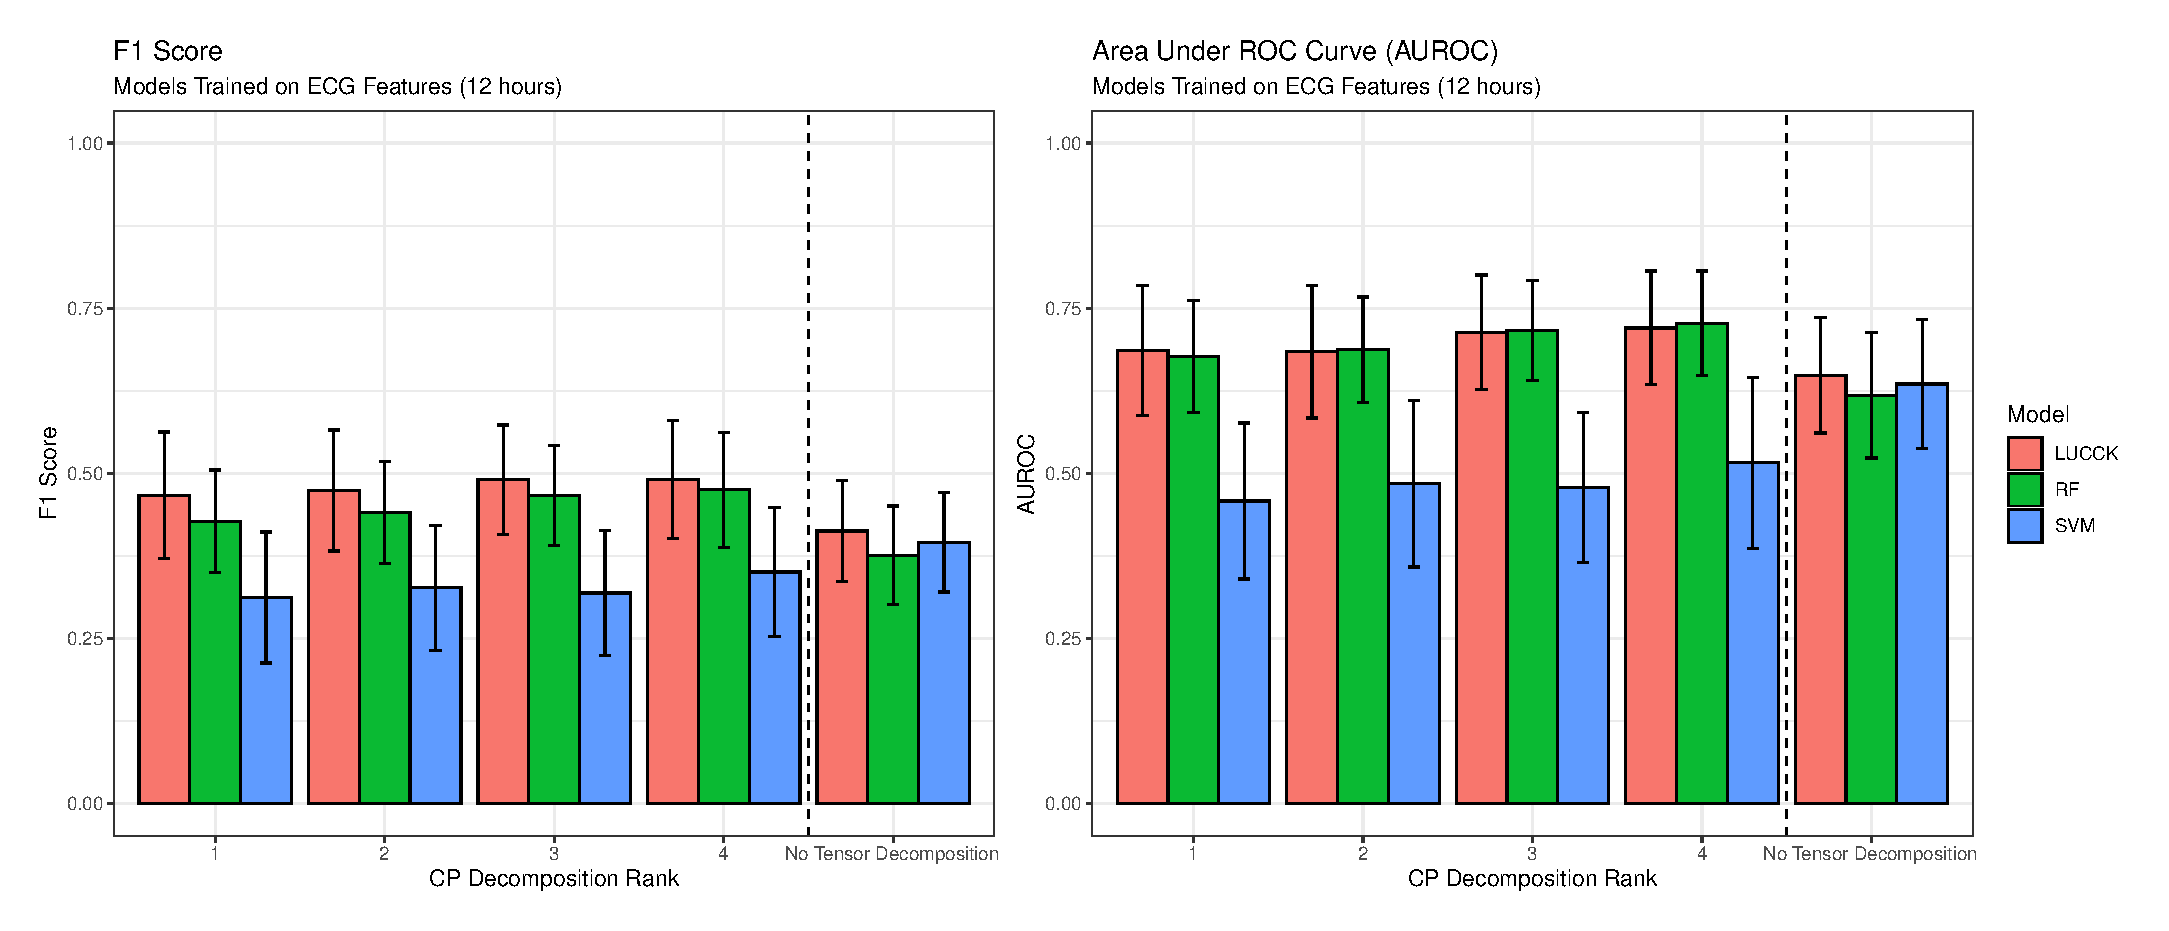
\includegraphics[width=\textwidth]{body/figures/ecg_12.eps}
        \caption{12-hour data}
    \end{subfigure}
    \caption{Models using ECG}
    \label{fig:ecgonly}
\end{figure}  % ECG 

\begin{figure}[htb]
    \centering
    \begin{subfigure}[htb]{\textwidth}
        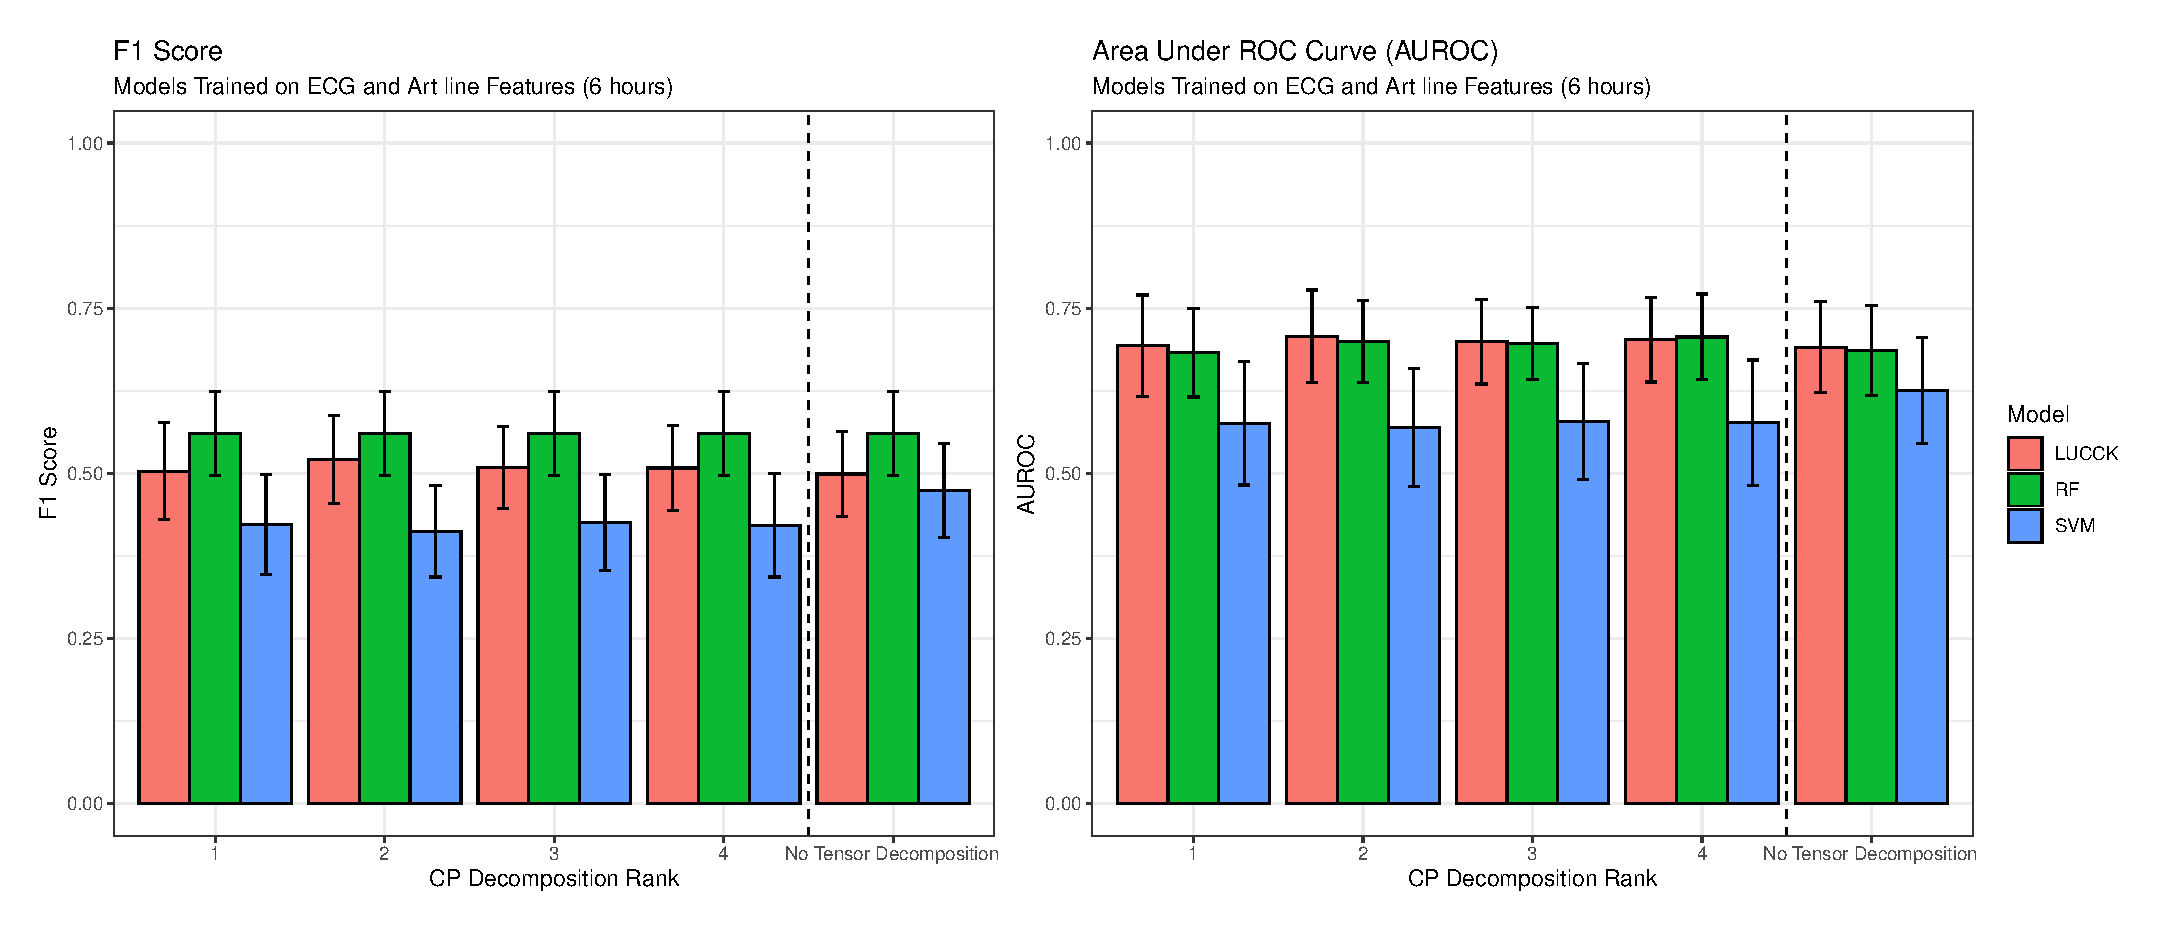
\includegraphics[width=\textwidth]{body/figures/both_6.eps}
        \caption{6-hour data}
    \end{subfigure}
    \hfill
    \begin{subfigure}[htb]{\textwidth}
        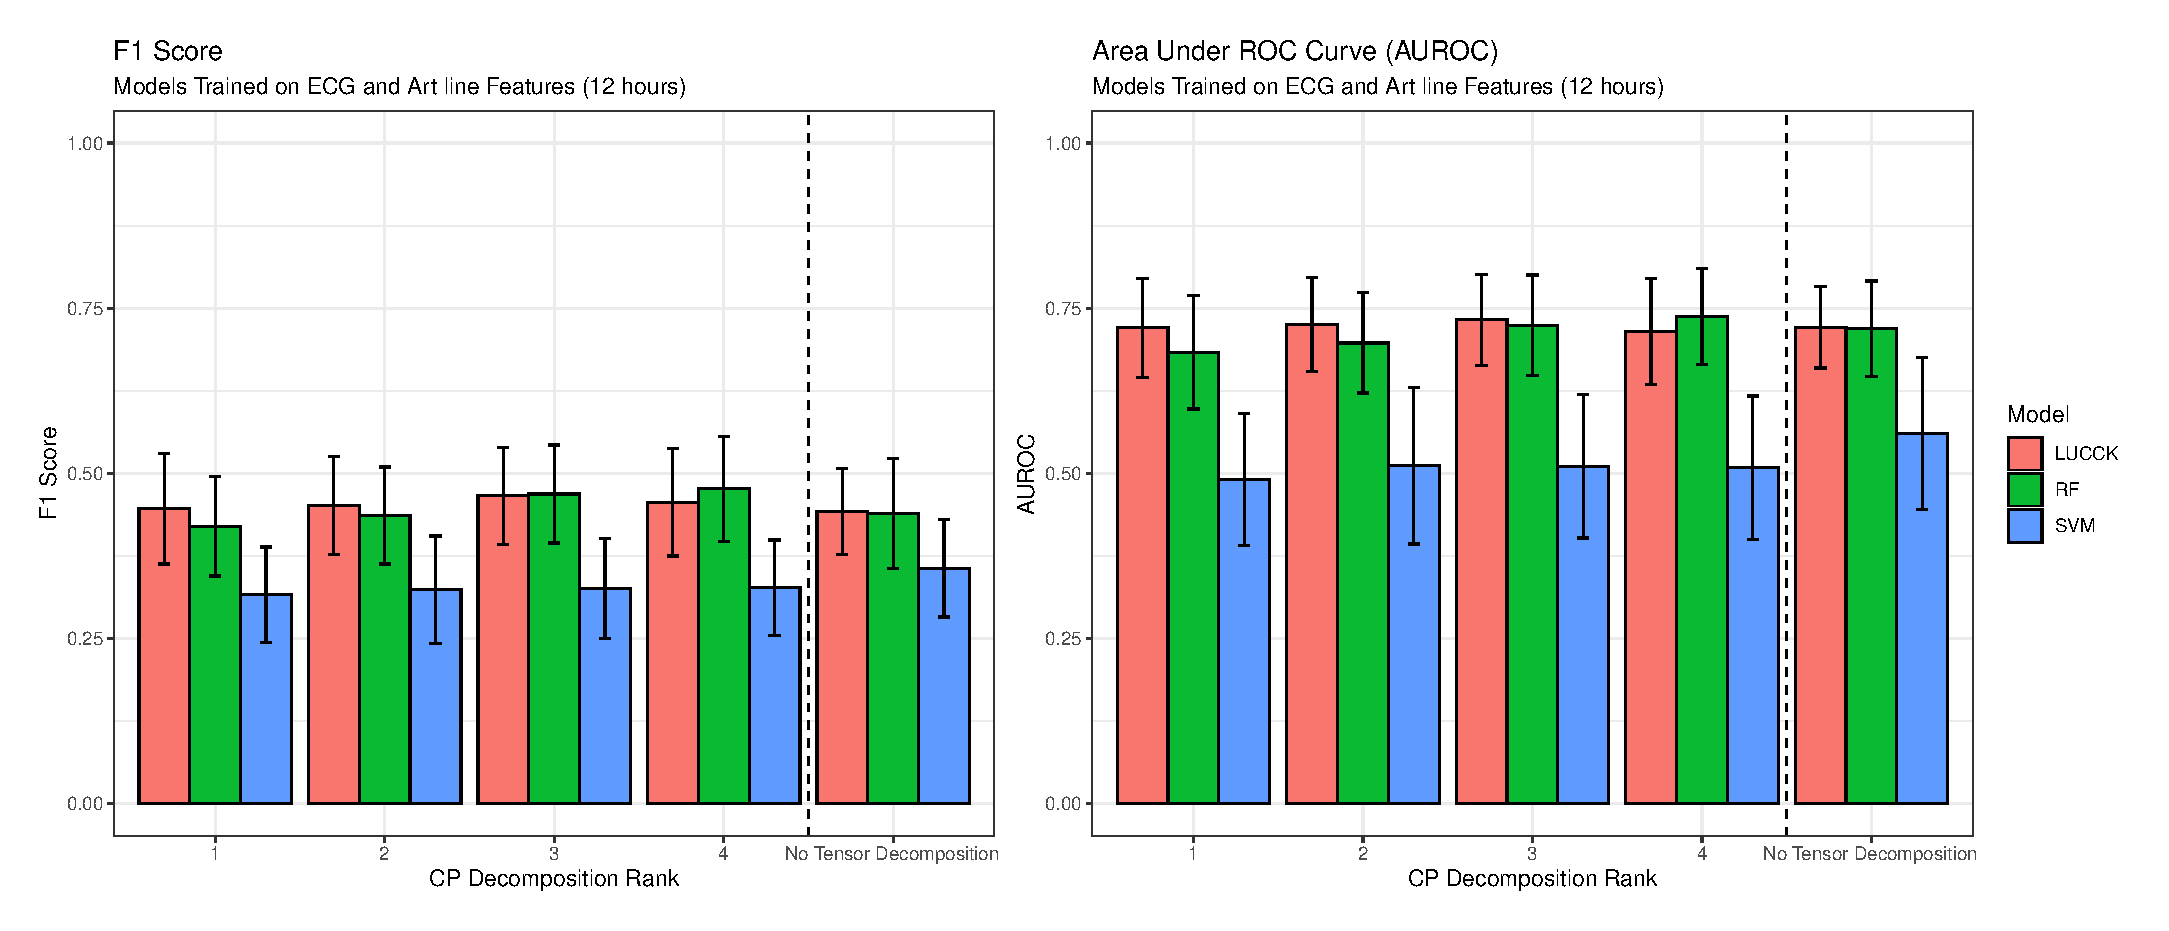
\includegraphics[width=\textwidth]{body/figures/both_12.eps}
        \caption{12-hour data}
    \end{subfigure}
    \caption{RF using Arterial Line and ECG}
    \label{fig:sigonly}
\end{figure}  % ART + ECG 

\begin{figure}[htb]
    \centering
    \begin{subfigure}[htb]{\textwidth}
        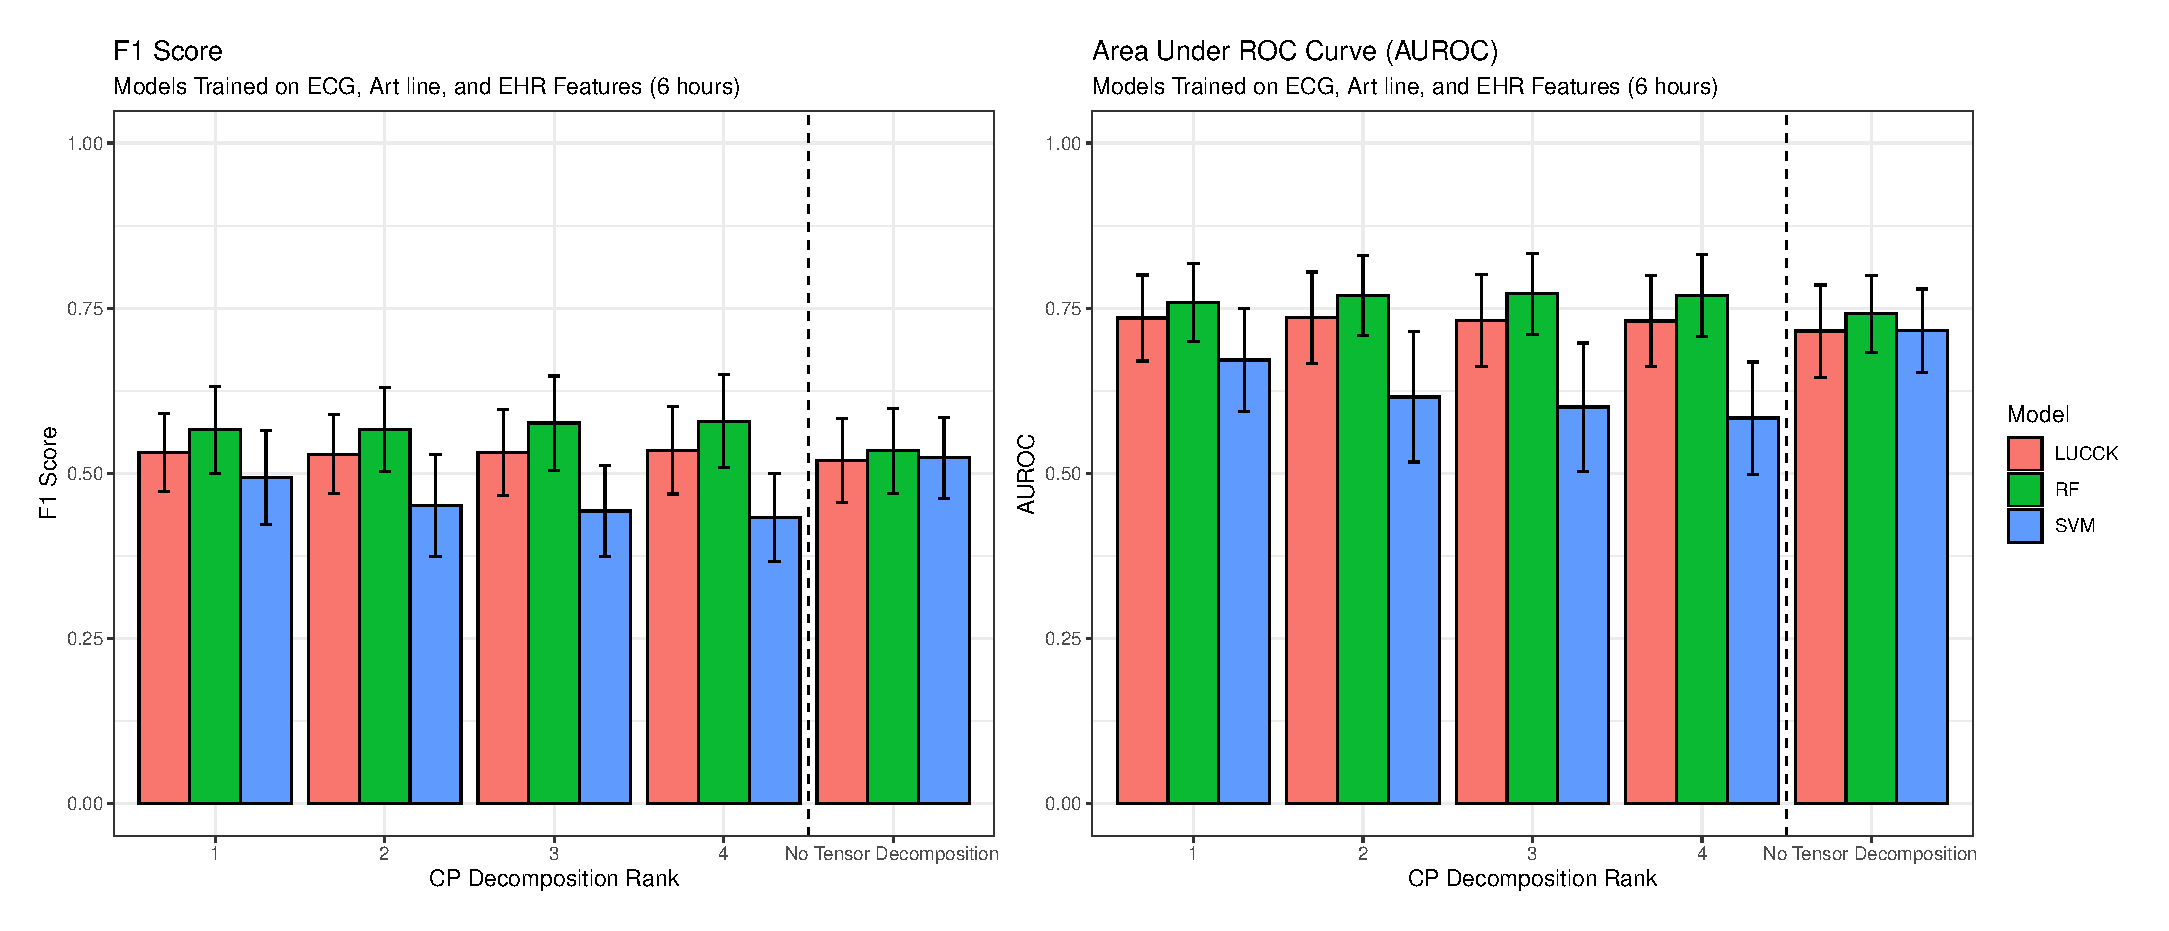
\includegraphics[width=\textwidth]{body/figures/all_6.eps}
        \caption{6-hour data}
    \end{subfigure}
    \hfill
    \begin{subfigure}[htb]{\textwidth}
        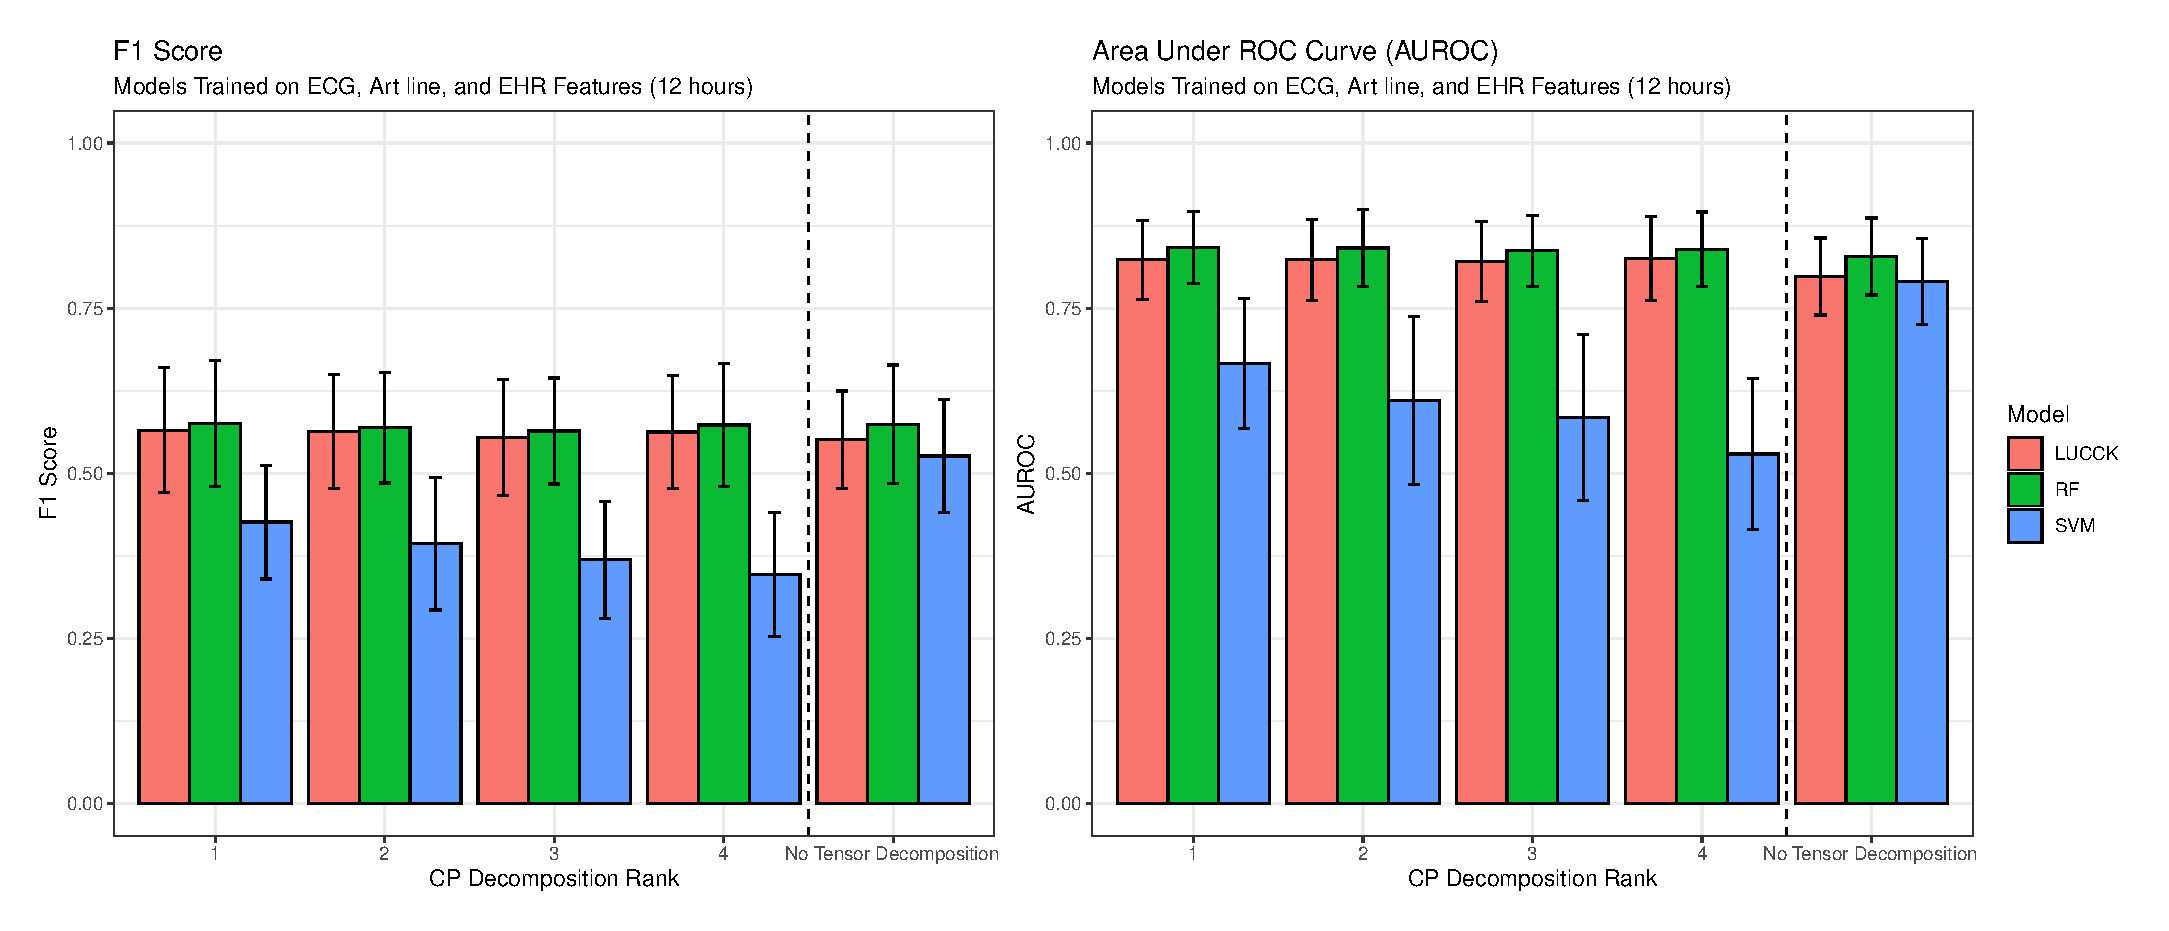
\includegraphics[width=\textwidth]{body/figures/all_12.eps}
        \caption{12-hour data}
    \end{subfigure}
    \caption{RF using Arterial Line, ECG, and EHR Data}
    \label{fig:sigEHR}
\end{figure}  % ART + ECG + EHR 



\begin{table}
    \centering
    \caption{ECG-Only Models, 6-hour gap}
    \begin{tabular}{|c|c|c|c|c|c|}
    \hline
        Model & Rank & F1 Score & Recall & Specificity & AUROC \\
        \hline
          & 1 & 0.4660 (0.0829) & 0.6279 (0.1231) & 0.6900 (0.1030) & 0.6146 (0.0888)\\
          & 2 & 0.4779 (0.0713) & 0.6792 (0.1136) & 0.6637 (0.0907) & 0.6421 (0.0849)\\
         LUCCK & 3 & 0.4785 (0.0663) & 0.6702 (0.1101) & 0.6749 (0.0793) & 0.6355 (0.0812)\\
          & \textbf{4} & \textbf{0.4844 (0.0650)} & 
         \textbf{0.6867 (0.1178)} & \textbf{0.6707 (0.0862)} & \textbf{0.6489 (0.0732)}\\
          & None & 0.4313 (0.0612) & 0.6606 (0.1259) & 0.5973 (0.1100) & 0.6038 (0.0735)\\
        \hline
         & 1 & 0.4551 (0.0554) & 0.6638 (0.1221) & 0.6397 (0.1084) & 0.6409 (0.0646)\\
          & 2 & 0.4743 (0.0548) & 0.7110 (0.0894) & 0.6269 (0.0956) & 0.6644 (0.0581)\\
         RF & 3 & 0.4665 (0.0558) & 0.6865 (0.1084) & 0.6391 (0.0885) & 0.6563 (0.0596)\\
          & \textbf{4} & \textbf{0.4839 (0.0558)} & \textbf{0.7197 (0.1041)} & \textbf{0.6384 (0.0908)} & \textbf{0.6690 (0.0644)}\\
          & None & 0.4080 (0.0570) & 0.6402 (0.1186) & 0.5699 (0.1113) & 0.5693 (0.0764)\\
        \hline
          & 1 & 0.3692 (0.0811) & 0.4950 (0.1462) & 0.6584 (0.1519) & 0.4863 (0.0955)\\
          & 2 & 0.3759 (0.0824) & 0.5202 (0.1379) & 0.6379 (0.1464) & 0.4963 (0.1014)\\
         SVM & 3 & 0.3819 (0.0848) & 0.5221 (0.1433) & 0.6560 (0.1082) & 0.5037 (0.1031)\\
          & 4 & 0.3806 (0.0899) & 0.5298 (0.1573) & 0.6435 (0.1225) & 0.4978 (0.1066)\\
          & \textbf{None} & \textbf{0.4409 (0.0661)} & \textbf{0.6361 (0.1151)} & \textbf{0.6342 (0.1364)} & \textbf{0.6205 (0.0859)}\\
        \hline                 
    \end{tabular}
\end{table}

\begin{table}
    \centering
    \caption{ECG-Only Models, 12-hour gap}
    \begin{tabular}{|c|c|c|c|c|c|}
        \hline
        Model & Rank & F1 Score & Recall & Specificity & AUROC \\
        \hline
         & 1 & 0.4667 (0.0956) & 0.6907 (0.1210) & 0.7421 (0.1136) & 0.6855 (0.0985)\\
         & 2 & 0.4739 (0.0916) & 0.6909 (0.1227) & 0.7534 (0.1104) & 0.6840 (0.1003)\\
        LUCCK & \textbf{3} & \textbf{0.4905 (0.0827)} & \textbf{0.7167 (0.1159)} & \textbf{0.7613 (0.0900)} & \textbf{0.7134 (0.0868)}\\
         & 4 & 0.4903 (0.0890) & 0.7300 (0.1158) & 0.7512 (0.0953) & 0.7200 (0.0861)\\
         & None & 0.4125 (0.0762) & 0.6700 (0.1267) & 0.6897 (0.0997) & 0.6485 (0.0876)\\
        \hline
        & 1 &  0.4270 (0.0779) & 0.6769 (0.1211) & 0.7039 (0.1107) & 0.6771 (0.0850)\\
         & 2 & 0.4405 (0.0775) & 0.7004 (0.1232) & 0.7085 (0.0978) & 0.6870 (0.0797)\\
        RF & 3 & 0.4661 (0.0754) & 0.7290 (0.1145) & 0.7242 (0.0930) & 0.7162 (0.0757)\\
         & \textbf{4} & \textbf{0.4750 (0.0870)} & \textbf{0.7318 (0.1155)} & \textbf{0.7331 (0.0902)} & \textbf{0.7272 (0.0791)}\\
         & None & 0.3756 (0.0749) & 0.6672 (0.1204) & 0.6253 (0.1240) & 0.6180 (0.0948)\\
         \hline
         & 1 & 0.3119 (0.0991) & 0.4740 (0.1565) & 0.6846 (0.1485) & 0.4580 (0.1180)\\
         & 2 & 0.3267 (0.0946) & 0.5204 (0.1637) & 0.6644 (0.1575) & 0.4842 (0.1263)\\
        SVM & 3 & 0.3188 (0.0946) & 0.5114 (0.1639) & 0.6671 (0.1429) & 0.4784 (0.1133)\\
         & 4 & 0.3505 (0.0975) & 0.5367 (0.1658) & 0.7013 (0.1217) & 0.5159 (0.1293)\\
         & \textbf{None} & \textbf{0.3954 (0.0751)} & \textbf{0.7027 (0.1390)} & \textbf{0.6318 (0.1348)} & \textbf{0.6351 (0.0972)}\\
        \hline
    \end{tabular}
\end{table}

\begin{table}
    \centering
    \caption{Models Trained on ECG and Art Line, 6-hour gap}
    \begin{tabular}{|c|c|c|c|c|c|}
        \hline
        Model & Rank & F1 Score & Recall & Specificity & AUROC \\
        \hline
         & 1 & 0.5030 (0.0734) & 0.7415 (0.1116) & 0.6467 (0.1154 & 0.6932 (0.0768)\\
         & \textbf{2} & \textbf{0.5206 (0.0666)} & \textbf{0.7208 (0.1022)} & \textbf{0.6947 (0.0985)} & \textbf{0.7073 (0.0700)}\\
        LUCCK & 3 & 0.5086 (0.0621) & 0.6913 (0.0972) & 0.7029 (0.0834) & 0.6992 (0.0642)\\
         & 4 & 0.5080 (0.0643) & 0.7181 (0.0987) & 0.6778 (0.0922) & 0.7021 (0.0641)\\
         & None & 0.4987 (0.0643) & 0.7346 (0.1112) & 0.6489 (0.1000) & 0.6906 (0.0689)\\
         \hline
         & 1 & 0.4911 (0.0608) & 0.7220 (0.1154) & 0.6470 (0.1089) & 0.6823 (0.0670)\\
         & 2 & 0.5070 (0.0571) & 0.7431 (0.0955) & 0.6554 (0.0949) & 0.6992 (0.0620)\\
         RF & 3 & 0.5069 (0.0551) & 0.7349 (0.1058) & 0.6664 (0.0762) & 0.6967 (0.0548)\\
         & \textbf{4} & \textbf{0.5197 (0.0633)} & \textbf{0.7510 (0.1033)} & \textbf{0.6707 (0.0860)} & \textbf{0.7064 (0.0650)}\\
         & None & 0.4894 (0.0632) & 0.7090 (0.0983) & 0.6552 (0.0936) & 0.6855 (0.0683)\\
         \hline
         & 1 & 0.4224 (0.0752) & 0.6102 (0.1489) & 0.6325 (0.1276) & 0.5756 (0.0933)\\
         & 2 & 0.4122 (0.0692) & 0.6139 (0.1370) & 0.6085 (0.1237) & 0.5693 (0.0897)\\
         SVM & 3 & 0.4258 (0.0728) & 0.6354 (0.1368) & 0.6099 (0.1223) & 0.5782 (0.0882)\\
         & 4 & 0.4214 (0.0787) & 0.6337 (0.1410) & 0.6038 (0.1217) & 0.5763 (0.0953)\\
         & \textbf{None} & \textbf{0.4738 (0.0709)} & \textbf{0.6995 (0.1336)} & \textbf{0.6370 (0.1179)} & \textbf{0.6250 (0.0804)}\\
         \hline
    \end{tabular}
\end{table}

\begin{table}
    \centering
    \caption{Models Trained on ECG and Art Line, 12-hour gap}
    \begin{tabular}{|c|c|c|c|c|c|c|}
        \hline
        Model & Rank & F1 Score & Recall & Specificity & AUROC \\
        \hline
         & 1 & 0.4461 (0.0834) & 0.7316 (0.1367) & 0.6854 (0.1402) & 0.7203 (0.0750)\\
         & 2 & 0.4515 (0.0740) & 0.7232 (0.1341) & 0.7068 (0.1144) & 0.7249 (0.0710)\\
        LUCCK & \textbf{3} & \textbf{0.4660 (0.0735)} & \textbf{0.7492 (0.1101)} & \textbf{0.7096 (0.1028)} & \textbf{0.7323 (0.0692)}\\
         & 4 & 0.4557 (0.0812) & 0.7309 (0.1265) & 0.7063 (0.1144) & 0.7149 (0.0804)\\
         & None & 0.4422 (0.0647) & 0.7692 (0.1214) & 0.6661 (0.0973) & 0.7208 (0.0615)\\
        \hline
         & 1 & 0.4199 (0.0756) & 0.7004 (0.1343) & 0.6766 (0.1188) & 0.6830 (0.0859)\\
         & 2 & 0.4360 (0.0735) & 0.7119 (0.1249) & 0.6937 (0.1046) & 0.6973 (0.0758)\\
        RF & 3 & 0.4686 (0.0741) & 0.7352 (0.1191) & 0.7225 (0.0981) & 0.7240 (0.0762)\\
         & \textbf{4} & \textbf{0.4763 (0.0792)} & \textbf{0.7546 (0.1040)} & \textbf{0.7182 (0.1015)} & \textbf{0.7375 (0.0724)}\\
         & None & 0.4389 (0.0829) & 0.7559 (0.1195) & 0.6661 (0.1014) & 0.7187 (0.0723)\\
        \hline
         & 1 & 0.3158 (0.0725) & 0.5650 (0.1687) & 0.6077 (0.1489) & 0.4907 (0.0997)\\
         & 2 & 0.3236 (0.0814) & 0.5734 (0.1773) & 0.6205 (0.1471) & 0.5113 (0.1186)\\
        SVM & 3 & 0.3251 (0.0757) & 0.5749 (0.1619) & 0.6142 (0.1568) & 0.5106 (0.1087)\\
         & 4 & 0.3268 (0.0721) & 0.5838 (0.1525) & 0.6072 (0.1494) & 0.5085 (0.1085)\\
         & \textbf{None} & \textbf{0.3561 (0.0737)} & \textbf{0.6461 (0.1580)} & \textbf{0.6114 (0.1465)} & \textbf{0.5604 (0.1151)}\\
         \hline
    \end{tabular}
\end{table}

\begin{table}
    \centering
    \caption{Models Trained on ECG, Art Line, and EHR Data, 6-hour gap}
    \begin{tabular}{|c|c|c|c|c|c|}
        \hline
        Model & Rank & F1 Score & Recall & Specificity & AUROC \\
        \hline
        & 1 & 0.5316 (0.0593) & 0.7390 (0.1081) & 0.6984 (0.0943) & 0.7351 (0.0652)\\
        & 2 & 0.5289 (0.0598) & 0.7398 (0.1043) & 0.6938 (0.0918) & 0.7354 (0.0692)\\
        LUCCK & 3 & 0.5312 (0.0653) & 0.7396 (0.1018) & 0.6970 (0.0878) & 0.7316 (0.0694)\\
        & \textbf{4} & \textbf{0.5347 (0.0661)} & \textbf{0.7410 (0.1108)} & \textbf{0.7025 (0.0846)} & \textbf{0.7305 (0.0689)}\\
        & None & 0.5190 (0.0636) & 0.7253 (0.1031) & 0.6912 (0.0811) & 0.7152 (0.0697)\\
        \hline
        & 1 & 0.5659 (0.0658) & 0.7569 (0.0908) & 0.7309 (0.0895) & 0.7581 (0.0592)\\
        & 2 & 0.5663 (0.0633) & 0.7740 (0.0757) & 0.7192 (0.0843) & 0.7686 (0.0606)\\
        RF & 3 & 0.5759 (0.0715) & 0.7691 (0.0921) & 0.7368 (0.0804) & 0.7716 (0.0613)\\
        & \textbf{4} & \textbf{0.5789 (0.0705)} & \textbf{0.7781 (0.0939)} & \textbf{0.7326 (0.0903)} & \textbf{0.7691 (0.0617)}\\
        & None & 0.5339 (0.0644) & 0.7560 (0.0892) & 0.6870 (0.0848) & 0.7413 (0.0587)\\
        \hline
        & 1 & 0.4935 (0.0712) & 0.6989 (0.1070) & 0.6700 (0.1017) & 0.6714 (0.0784)\\
        & 2 & 0.4509 (0.0775) & 0.6589 (0.1266) & 0.6321 (0.1164) & 0.6155 (0.0986)\\
        SVM & 3 & 0.4428 (0.0692) & 0.6504 (0.1244) & 0.6264 (0.1165) & 0.6002 (0.0970)\\
        & 4 & 0.4331 (0.0669) & 0.6310 (0.1184) & 0.6288 (0.1113) & 0.5835 (0.0851)\\
        & \textbf{None} & \textbf{0.5234 (0.0613)} & \textbf{0.7374 (0.0970)} & \textbf{0.6881 (0.0753)} & \textbf{0.7156 (0.0633)}\\
        \hline
    \end{tabular}
\end{table}

\begin{table}
    \centering
    \caption{Models Trained on ECG, Art Line, and EHR Data, 12-hour gap}
    \begin{tabularx}{\textwidth}{|C|C|C|C|C|C|}
        \hline
        Model & Rank & F1 Score & Recall & Specificity & AUROC \\
        \hline
        & \textbf{1} & \textbf{0.5650 (0.0947)} & \textbf{0.8167 (0.0879)} & \textbf{0.7827 (0.0916)} & \textbf{0.8233 (0.0598)}\\
        & 2 & 0.5633 (0.0865) & 0.8043 (0.0911) & 0.7896 (0.0838) & 0.8233 (0.0613)\\
        LUCCK & 3 & 0.5543 (0.0875) & 0.8119 (0.0822) & 0.7762 (0.0842) & 0.8210 (0.0607)\\
        & 4 & 0.5625 (0.0852) & 0.8274 (0.0918) & 0.7781 (0.0839) & 0.8256 (0.0635)\\
        & None & 0.5505 (0.0739) & 0.8057 (0.0973) & 0.7794 (0.0750) & 0.7979 (0.0584)\\
        \hline                
        & \textbf{1} & \textbf{0.5754 (0.0952)} & \textbf{0.8187 (0.1039)} & \textbf{0.7936 (0.0830)} & \textbf{0.8418 (0.0541)}\\
        & 2 & 0.5691 (0.0840) & 0.8046 (0.0901) & 0.7972 (0.0721) & 0.8412 (0.0580)\\
        RF & 3 & 0.5639 (0.0803) & 0.8263 (0.1022) & 0.7822 (0.0722) & 0.8370 (0.0538)\\
        & 4 & 0.5731 (0.0927) & 0.8310 (0.0901) & 0.7847 (0.0876) & 0.8390 (0.0567)\\
        & None & 0.5743 (0.0896) & 0.8454 (0.0886) & 0.7791 (0.0871) & 0.8282 (0.0582)\\
        \hline
        & 1 & 0.4261 (0.0861) & 0.7126 (0.1360) & 0.6805 (0.0901) & 0.6660 (0.0984)\\
        & 2 & 0.3934 (0.1005) & 0.6728 (0.1521) & 0.6490 (0.1337) & 0.6104 (0.1270)\\
        SVM & 3 & 0.3689 (0.0886) & 0.6441 (0.1608) & 0.6389 (0.1176) & 0.5839 (0.1257)\\
        & 4 & 0.3470 (0.0941) & 0.5982 (0.1510) & 0.6280 (0.1465) & 0.5290 (0.1142)\\
        & \textbf{None} & \textbf{0.5261 (0.0856)} & \textbf{0.8033 (0.1041)} & \textbf{0.7505 (0.0922)} & \textbf{0.7901 (0.0654)}\\
        \hline
    \end{tabularx} 
\end{table}


\clearpage